
\section{Image Handling in Python}

\begin{minted}[tabsize=2]{python}
plt.imshow(np.hstack((im_float, im_float)), cmap="gray", vmin=0, vmax=1);
\end{minted}

\begin{center}
	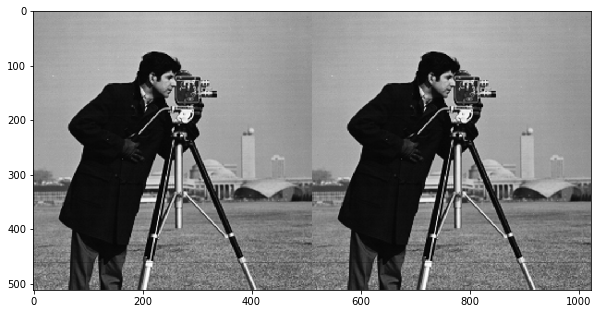
\includegraphics[width=0.7\linewidth]{img/hstack_image}
\end{center}

\subsection{Fading an Image}
\begin{minted}[tabsize=2]{python}
im = skimage.io.imread("data/snoopy.png")
im = im/255 # tip: use floating point values

ims = []

im_temp = np.fliplr(im)
ims.append(im_temp)
for i in range(1,5):
	im_temp = im_temp + (0.4)**i
	ims.append(im_temp)

plt.imshow(np.hstack(ims),vmin=0, vmax=1, cmap="gray")
\end{minted}

\begin{center}
	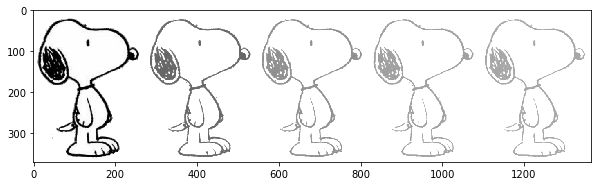
\includegraphics[width=0.7\linewidth]{img/snoopy_fade}
\end{center}

\subsubsection{IPyWidgets}
\begin{minted}[tabsize=2]{python}
@interact(thresh=widgets.FloatSlider(min=0.0, max=0.5, step=0.01, value=0.2))
def threshold(thresh):
	im_thresh = []
	for line in im:
		im_thresh.append([pixel if pixel > np.min(line)
			+ thresh else float(0) for pixel in line])
	plt.imshow(im_thresh, cmap="gray", vmin=0, vmax=1)
	plt.show()
\end{minted}

\begin{center}
	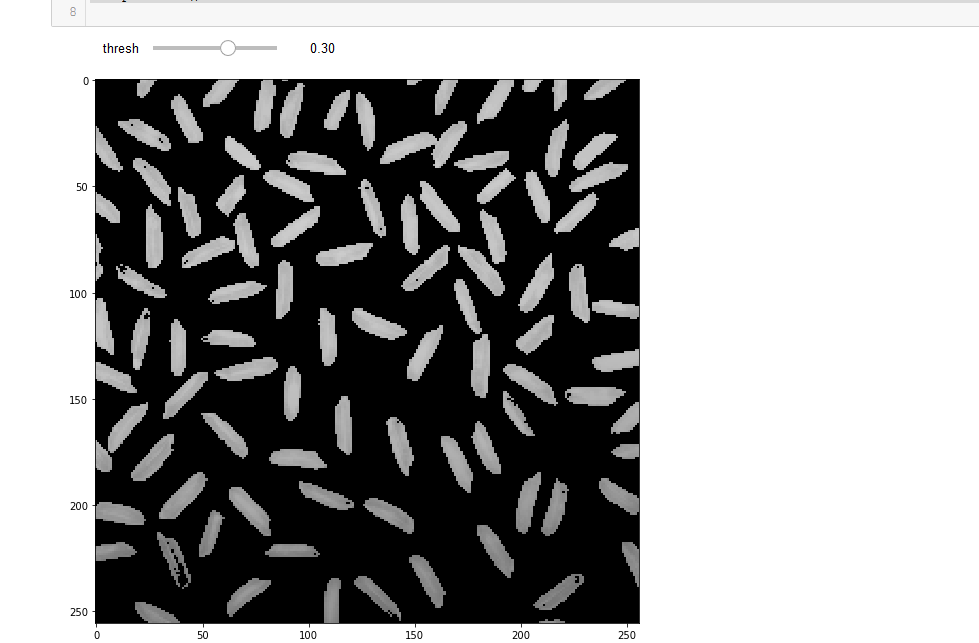
\includegraphics[width=0.6\linewidth]{img/ipywidgets_example}
\end{center}
